\documentclass[a4paper,12pt,twoside]{memoir}
\usepackage{longtable}
\usepackage{btp}    % Use the trainermanual package option (i.e. \usepackage[trainermanual]{btp}) to generate the Trainer's version of the manual
%\usepackage[
%  noinfo,
%  cam,
%  cross,                % crosses as marks
%  a4,
%  width=6.25in,         % the width of the galley
%  height=9.25in,        % the height of the galley
%  center                % actual page is centered on the galley
%]{crop}

\usepackage{tikz}
\usetikzlibrary{shapes,arrows}

% Set some Workshop specific info
\setWorkshopTitle{Biotech 7005: Practical Manual\\[5mm]
Introduction To NGS Data \\ [5mm]
\& Analytic Tools}
\setWorkshopVenue{Bioinformatics Hub\newline
University of Adelaide}
\setWorkshopDate{\today}
\setWorkshopAuthor{
}

\begin{document}

%
% Workshop Title Page
%
\workshoptitlepage

%
% CC-BY
%
\input{licences/licence.tex}
\clearpage

\tableofcontents

\chapter{Workshop Information}
\clearpage

%
% Trainers Page
%
\section{The Demonstrators}

\newlength{\trainerIconWidth}
\setlength{\trainerIconWidth}{2.0cm}

\begin{center}
\begin{longtable}{>{\centering\arraybackslash} m{1.1\trainerIconWidth} m{1\textwidth}}

  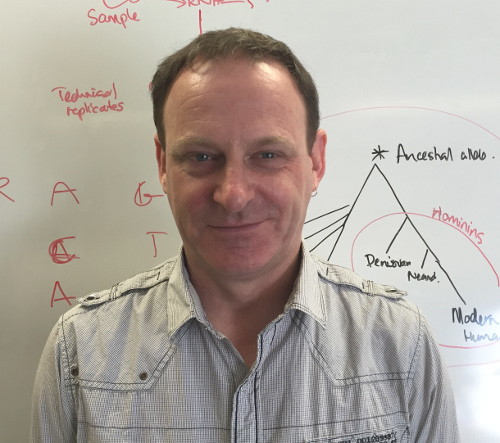
\includegraphics[width=\trainerIconWidth]{photos/steveped.jpeg} &
    \textbf{Mr. Steve Pederson}\newline
    Co-ordinator\newline
    Bioinformatics Hub\newline
    The University of Adelaide\newline
    South Australia\newline
    \mailto{stephen.pederson@adelaide.edu.au}\\
     \\

    
  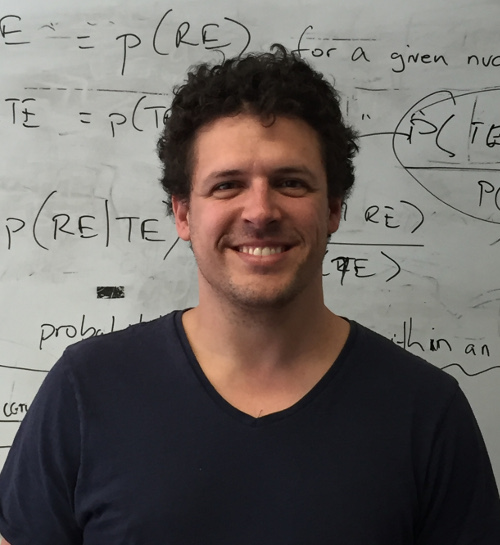
\includegraphics[width=\trainerIconWidth]{photos/jimmyb.jpg} &
    \textbf{Dr. Jimmy Breen}\newline
    Bioinformatician\newline
    Bioinformatics Hub \& Robinson Research Institute\newline
    The University of Adelaide\newline
    South Australia\newline
    \mailto{jimmy.breen@adelaide.edu.au}\\
    \\
    
     &
    \textbf{Dr. Dan Kortschak}\newline
    Bioinformatician\newline
    Adelson Research Group\newline
    The University of Adelaide\newline
    South Australia\newline
    \mailto{dan.kortschak@adelaide.edu.au}\\
  
\end{longtable}
\end{center}



%
% Workshop Preamble
%
%
% Start: General Information describing the workshop and the structure of the handouts
%
\newpage

\section{Course Summary}
In these practical sessions we will be introducing you to a small number of the basic tools required for NGS data handling, as well as giving you a basic familiarity with what the data actually looks like.
Whilst we will not be able to cover all of the rich \& diverse set of tools available, we hope to cover many of the key concepts \& questions to ask of your data, as well as give you an understanding of what information is actually in the data.\\

Whilst most of the session will involve looking at individual files, in reality most of our analysis will be performed using some type of script to automate, \& easily reproduce an analysis. \\

These sessions are also intended to explore several tools in actual detail, rather than rush across the whole field.
There is large amount of information that we won't have time to discuss, but hopefully some important tools and thought processes will be covered \& enable you make better progress with your own datasets.\\

We'd also encourage you to sign up for some of the high-traffic websites like \textit{BioStars} or \textit{SEQanswers} as these are a rich resource for your own problem solving.\\


\begin{warning}
While you could fly through the hands-on sessions doing copy-and-paste, you will learn more if you take the time to enter the commands and take the time to understand what each command is doing! \\

The questions in the manual don't need to be submitted for assessment.
However it is still highly important that you answer these questions as they will greatly assist your understanding of the processes involved.
\end{warning}

The commands to enter at a terminal look something like this:
\begin{lstlisting}
tophat --solexa-quals -g 2 --library-type fr-unstranded -j annotation/Danio_rerio.Zv9.66.spliceSites -o tophat/ZV9_2cells genome/ZV9 data/2cells_1.fastq data/2cells_2.fastq
\end{lstlisting}  

The following styled code is not to be entered at a terminal, it is simply to show you the syntax of
the command. You must use your own judgement to substitute in the correct arguments, options,
filenames etc

\begin{lstlisting}[style=command_syntax]
tophat [options]* <index_base> <reads_1> <reads_2>
\end{lstlisting}

The following icons are used in the margin, throughout the documentation to help you navigate around
the document more easily:

% TODO limit the use of some icons throughout as some are clearly overused and confuse the eye
\hspace*{.2cm}\vcent{\includegraphics[height=1cm]{icons/info.png}} Important\\
\hspace*{.2cm}\vcent{\includegraphics[height=1cm]{icons/notes.png}} For reference\\
\hspace*{.2cm}\vcent{\includegraphics[height=1cm]{icons/steps.png}} Follow these steps\\
\hspace*{.2cm}\vcent{\includegraphics[height=1cm]{icons/questions.png}} Questions to answer\\
\hspace*{.2cm}\vcent{\includegraphics[height=1cm]{icons/warning.png}} Warning - STOP and read\\

\subsubsection*{Today's Notes}
Today's notes are also available electronically from the site \url{http://uofabioinformaticshub.github.io/NGS\_Practical}

\clearpage
%\input{016_computer_setup/setup.tex}

%
% Start of modules
% Switch chapter styling to module
%
\chapterstyle{module}


%
% End of modules
% Switch back to normal workshop chapter styling
%
\chapterstyle{workshop}

\chapter{Space for Personal Notes or Feedback}
\clearpage

%
% Some empty ruled comments pages
%
\myruledpage{0cm}{1cm}
\myruledpage{0cm}{1cm}

\end{document}
